%
% This is a borrowed LaTeX template file for lecture notes for CS267,
% Applications of Parallel Computing, UCBerkeley EECS Department.
%

\documentclass{article}
\usepackage{titlesec}
%\setlength{\oddsidemargin}{0.25 in}
%\setlength{\evensidemargin}{-0.25 in}
\setlength{\oddsidemargin}{0 in}
\setlength{\evensidemargin}{0 in}
\setlength{\topmargin}{-0.6 in}
\setlength{\textwidth}{6.5 in}
\setlength{\textheight}{8.5 in}
\setlength{\headsep}{0.75 in}
\setlength{\parindent}{0 in}
\setlength{\parskip}{0.1 in}


%
% ADD PACKAGES here:
%

\usepackage{amssymb}	% Already loads amsfonts
\usepackage{amsthm}
\usepackage{graphicx}
\usepackage{mathtools}	% Already loads amsmath
\usepackage{hyperref}
\usepackage{enumitem}
\usepackage{clrscode3e}  % for typesetting pseudocode
\usepackage{ulem}
\usepackage[usenames,dvipsnames]{xcolor}
\usepackage{multicol}


% Tikz and setup
\usepackage{tikz}
\usepackage{tikz-cd}
\usetikzlibrary{intersections, angles, quotes, calc, positioning}
\usetikzlibrary{arrows.meta}
\usepackage{pgfplots}
\pgfplotsset{compat=1.13}


\tikzset{
    force/.style={thick, {Circle[length=2pt]}-stealth, shorten <=-1pt}
}

%
% The following commands set up the lecnum (lecture number)
% counter and make various numbering schemes work relative
% to the lecture number.
%
\newcounter{lecnum}
\renewcommand{\thepage}{\thelecnum-\arabic{page}}
\renewcommand{\thesection}{\thelecnum.\arabic{section}}
\renewcommand{\theequation}{\thelecnum.\arabic{equation}}
\renewcommand{\thefigure}{\thelecnum.\arabic{figure}}
\renewcommand{\thetable}{\thelecnum.\arabic{table}}

%
% The following macro is used to generate the header.
%
\newcommand{\lecture}[5]{
   \pagestyle{myheadings}
   \thispagestyle{plain}
   \newpage
   \setcounter{lecnum}{#2}
   \setcounter{page}{1}
   \noindent
   \begin{center}
   \framebox{
      \vbox{\vspace{2mm}
    \hbox to 6.28in { {\bf #1
	\hfill} }
       \vspace{4mm}
       \hbox to 6.28in { {\Large \hfill Lecture #2: #3  \hfill} }
       \vspace{2mm}
       \hbox to 6.28in { {\it Lecturer: #4 \hfill Scribe: #5} }
      \vspace{2mm}}
   }
   \end{center}
   \markboth{Lecture #2: #3}{Lecture #2: #3}
   \vspace*{4mm}
}
\renewcommand{\cite}[1]{[#1]}
\def\beginrefs{\begin{list}%
        {[\arabic{equation}]}{\usecounter{equation}
         \setlength{\leftmargin}{2.0truecm}\setlength{\labelsep}{0.4truecm}%
         \setlength{\labelwidth}{1.6truecm}}}
\def\endrefs{\end{list}}
\def\bibentry#1{\item[\hbox{[#1]}]}

\newcommand{\fig}[3]{
			\vspace{#2}
			\begin{center}
			Figure \thelecnum.#1:~#3
			\end{center}
	}

% Colored theorem styles
\makeatother
\usepackage{thmtools}
\usepackage[framemethod=TikZ]{mdframed}
\mdfsetup{skipabove=1em,skipbelow=1em}

\declaretheoremstyle[
    headfont=\bfseries\sffamily\color{ForestGreen!70!black}, bodyfont=\normalfont,
    mdframed={
        linewidth=2pt,
        rightline=false, topline=false, bottomline=false,
        linecolor=ForestGreen, backgroundcolor=ForestGreen!5,
    },
    spaceabove=8pt
]{thmgreenbox}

\declaretheoremstyle[
    headfont=\bfseries\sffamily\color{NavyBlue!70!black}, bodyfont=\normalfont,
    mdframed={
        linewidth=2pt,
        rightline=false, topline=false, bottomline=false,
        linecolor=NavyBlue, backgroundcolor=NavyBlue!5,
    },
    spaceabove=8pt
]{thmbluebox}

\declaretheoremstyle[
    headfont=\bfseries\sffamily\color{NavyBlue!70!black}, bodyfont=\normalfont,
    mdframed={
        linewidth=2pt,
        rightline=false, topline=false, bottomline=false,
        linecolor=NavyBlue
    },
    spaceabove=8pt
]{thmblueline}

\declaretheoremstyle[
    headfont=\bfseries\sffamily\color{RawSienna!70!black}, bodyfont=\normalfont,
    mdframed={
        linewidth=2pt,
        rightline=false, topline=false, bottomline=false,
        linecolor=RawSienna, backgroundcolor=RawSienna!5,
    },
    spaceabove=8pt
]{thmredbox}

\declaretheoremstyle[
    headfont=\bfseries\sffamily\color{RawSienna!70!black}, bodyfont=\normalfont,
    numbered=no,
    mdframed={
        linewidth=2pt,
        rightline=false, topline=false, bottomline=false,
        linecolor=RawSienna, backgroundcolor=RawSienna!1,
    },
    qed=\qedsymbol,
    spaceabove=8pt
]{thmproofbox}

\declaretheoremstyle[
    headfont=\bfseries\sffamily\color{NavyBlue!70!black}, bodyfont=\normalfont,
    numbered=no,
    mdframed={
        linewidth=2pt,
        rightline=false, topline=false, bottomline=false,
        linecolor=NavyBlue, backgroundcolor=NavyBlue!1,
    },
    spaceabove=8pt
]{thmexplanationbox}

% Use these for theorems, lemmas, proofs, etc.
\theoremstyle{definition}
\declaretheorem[style=thmgreenbox, name=Definition, numberwithin=lecnum]{definition}
\declaretheorem[style=thmbluebox, numbered=no, name=Example]{example}
\declaretheorem[style=thmredbox, name=Theorem, numberwithin=lecnum]{theorem}
\declaretheorem[style=thmredbox, name=Proposition, sibling=theorem]{proposition}
\declaretheorem[style=thmredbox, name=Lemma, sibling=theorem]{lemma}
\declaretheorem[style=thmredbox, name=Corollary, sibling=theorem]{corollary}
% \newtheorem{theorem}{Theorem}[lecnum]
% \newtheorem{lemma}[theorem]{Lemma}
% \newtheorem{claim}[theorem]{Claim}
% \newtheorem{corollary}[theorem]{Corollary}
% \newtheorem{definition}[theorem]{Definition}
\declaretheorem[style=thmblueline, numbered=no, name=Remark]{remark}
\renewenvironment{proof}{{\bf \textit{Proof.}}}{\hfill\rule{2mm}{2mm}}
\makeatletter


% **** IF YOU WANT TO DEFINE ADDITIONAL MACROS FOR YOURSELF, PUT THEM HERE:

\renewcommand\Pr{\mathbb{P}}
\newcommand\Ex{\mathbb{E}}

\newcommand\N{\mathbb{N}}
\newcommand\Z{\mathbb{Z}}
\newcommand\Q{\mathbb{Q}}
\newcommand\R{\mathbb{R}}
\newcommand\C{\mathbb{C}}
\newcommand\F{\mathbb{F}}

\DeclarePairedDelimiter\ceil{\lceil}{\rceil}
\DeclarePairedDelimiter\floor{\lfloor}{\rfloor}
\DeclarePairedDelimiter\anglebrac{\langle}{\rangle}

\begin{document}
\lecture{MAT344 Intro to Combinatorics}{9}{Planarity and Euler's Formula}{Keegan Dasilva Barbosa}{Kevin Gao}

\section{Planarity}

\begin{definition}[Planarity]
    We say a graph $G$ is \textit{\textbf{planar}} if there \textbf{exists} a depiction of it on a plane without any edge crossing.
\end{definition}

To put in simple terms, a graph is planar if one can draw the graph on a piece of paper without any edge crossing each other. The definition as it is presented here is quite vague and lack mathematical rigor. Thankfully, this is formalized with a theorem by Kuratowski that we will introduce later that presents an equivalence to our definition of planarity.

There are many practical applications of graph planarity. In computer science, there is a notion of thickness that correlates planarity to how difficult it is to embed a network. Planarity is also related to integrated circuit design in cases when lines or wires are not allowed to cross.

\begin{theorem}[Four Color Theorem]
    Every planar graph has chromatic number of at most 4.
\end{theorem}

The proof of the Four Color theorem relies on brute-force computation methods and was only completed 1976. It is complex and not very readable, so we will not provide the proof here but instead treat it as a proven fact.

The Four Color Theorem implies that if $G$ is planar, $\chi(G) \leq 4$, so any graph with $\chi(G) \geq 5$ cannot be planar.

\begin{corollary}
    Any graph containing a copy of $K_5$ cannot be planar.
\end{corollary}

\subsection{Face}

Roughly speaking, a \textit{\textbf{face}} (in context of graph theory) is a region not containing other vertices or edges, bounded by edges of a graph in its planar depiction. Note that when discussing the \textbf{number of faces}, it is important to only consider the \textbf{planar depiction} of a graph because otherwise we can create arbitrary many faces.

\begin{figure}[htbp]
    \centering
    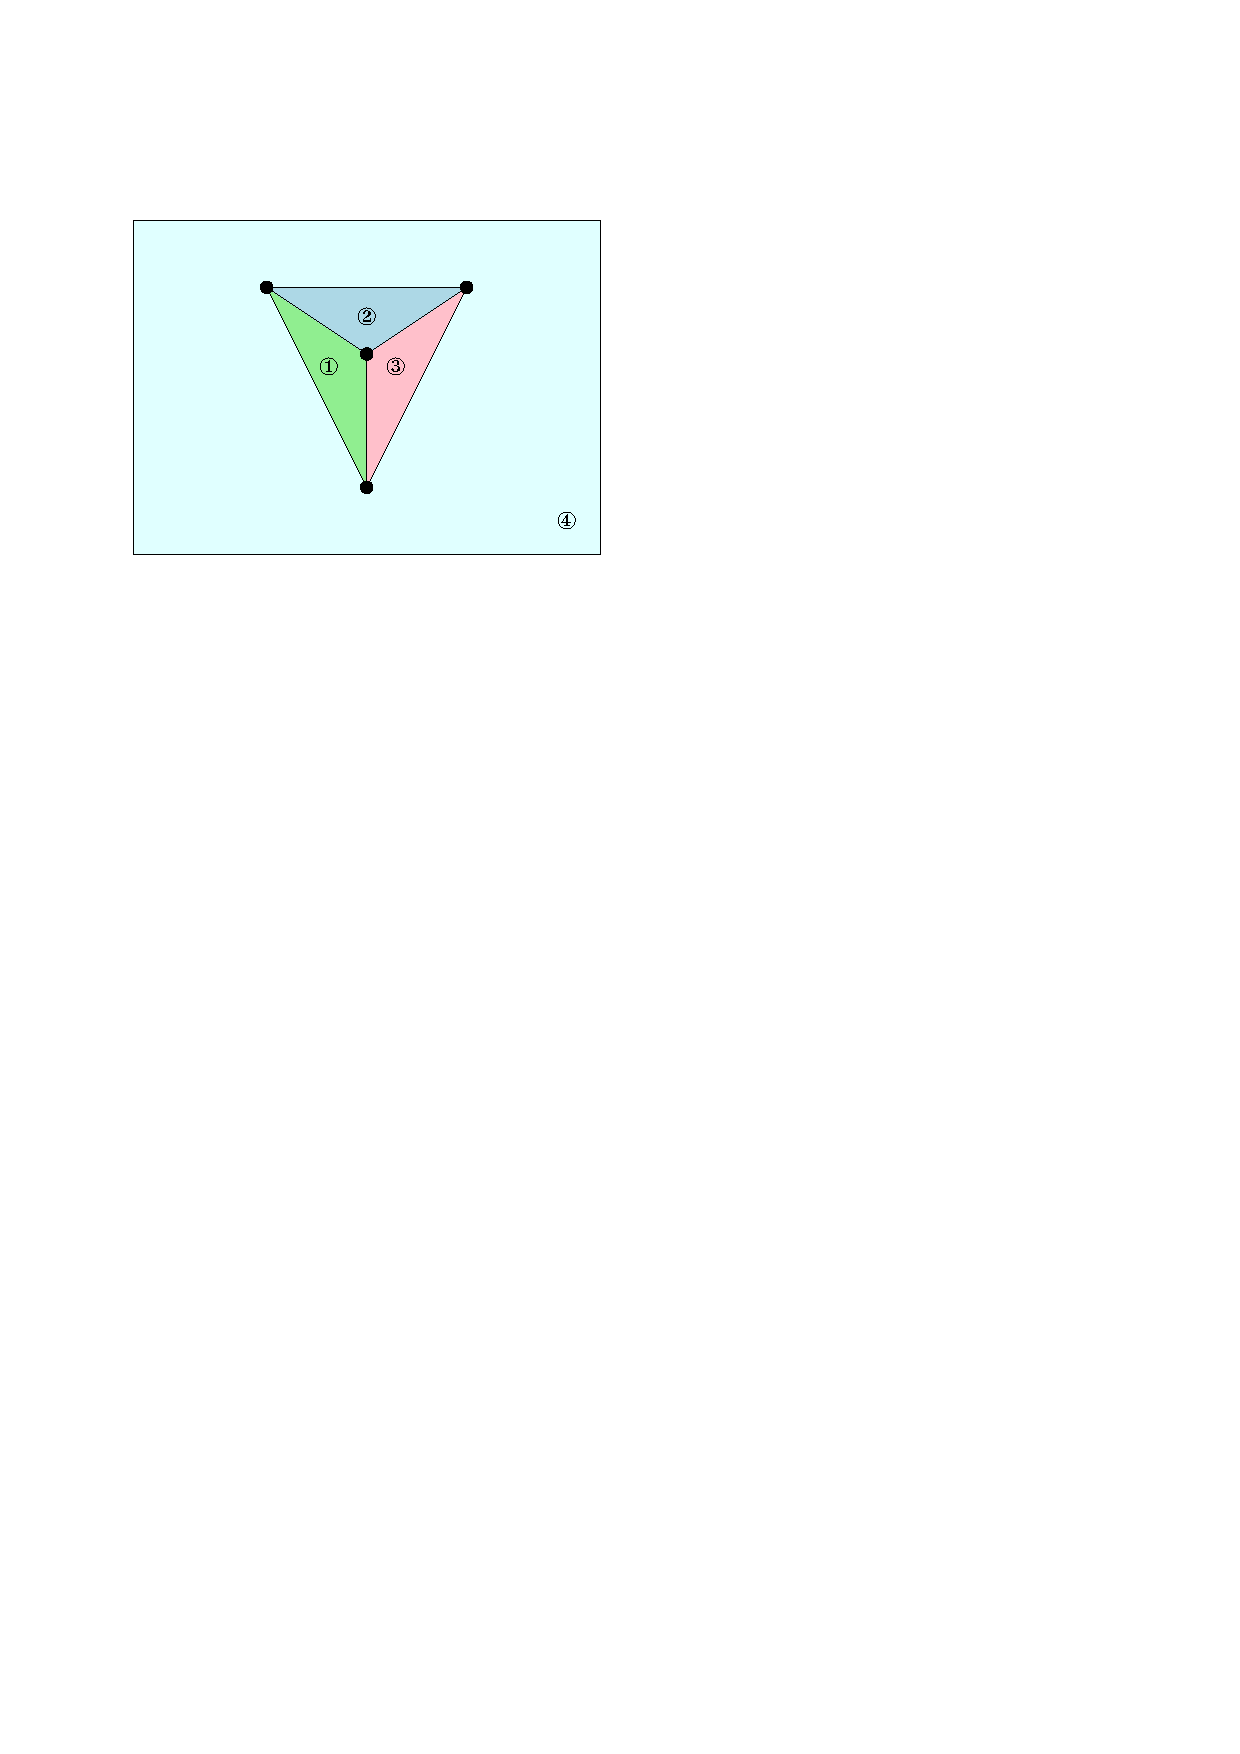
\includegraphics[width=0.4\linewidth]{figures/planar-graph-faces.pdf}
    \caption{A planar graph and its 4 faces.}
    \label{fig:planar-graph-faces}
\end{figure}

Is there any pattern between the number of vertices, edges, and faces in a planar graph? Consider the graph shown in Figure \ref{fig:planar-graph-faces}. We have 4 edges, 6 vertices, and 4 faces.

The triangle graph $K_3$ (complete graph of 3 vertices) has 3 vertices, 3 edges, and 2 faces. The path graph of $n$ vertices $P_n$ have $n$ vertices, $n-1$ edges, and one face. The cycle graph of $n$ vertices $C_n$ has $n$ vertices, $n$ edges, and 2 faces. See Figure \ref{fig:euler-formula-example-graphs}

\begin{figure}[htbp]
    \centering
    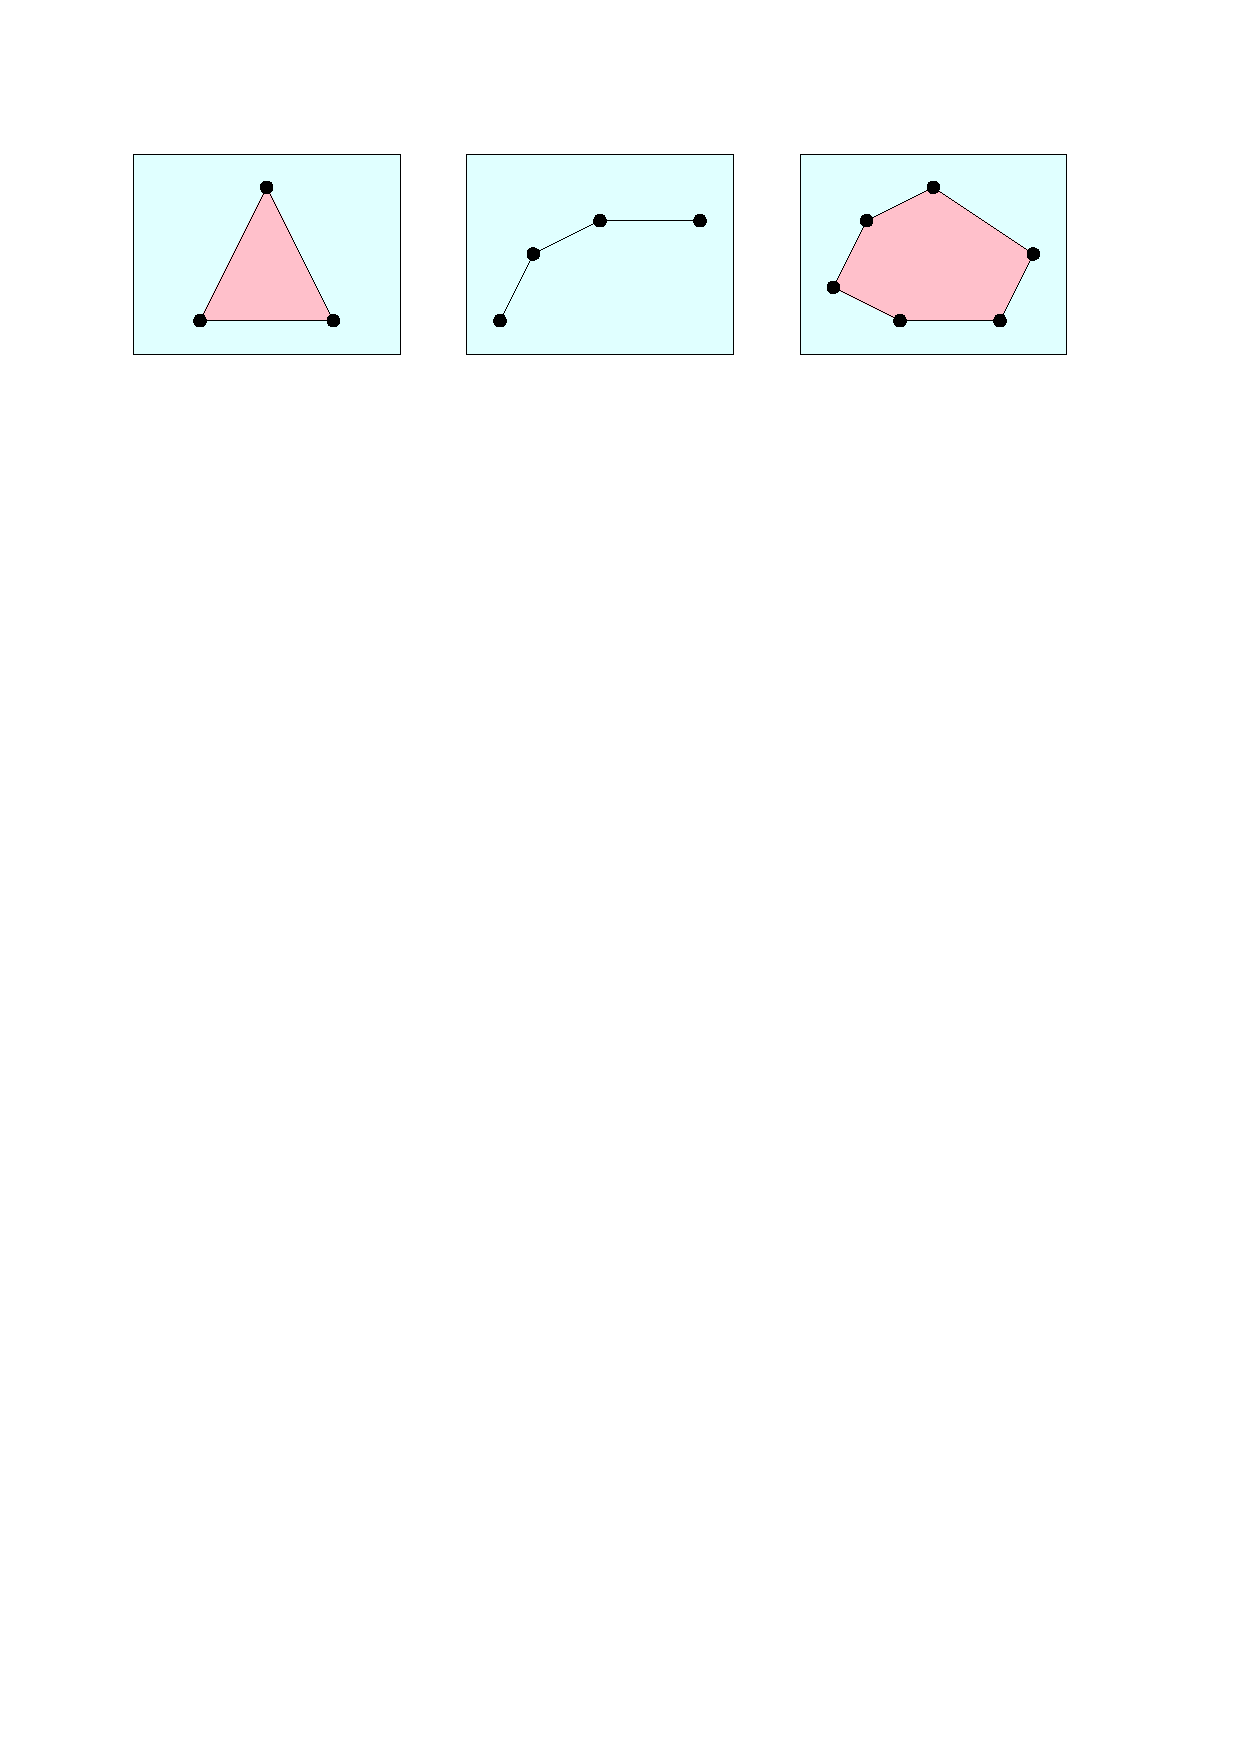
\includegraphics[width=0.6\linewidth]{figures/euler-formula-example-graphs.pdf}
    \caption{The triangle graph $K_3$, path graph $P_n$, and cycle graph $C_n$.}
    \label{fig:euler-formula-example-graphs}
\end{figure}

\section{Euler's Formula}

From the previous examples (Figure \ref{fig:planar-graph-faces} and \ref{fig:euler-formula-example-graphs}), we know there is some relationship between the number of vertices, edges, and faces in a planar depiction of a graph. This pattern is characterized by Euler's formula:

\begin{theorem}[Euler's Formula for Planar Graphs]
    Let $G$ be a connected planar graph with $n$ vertices, $m$ edges, and $f$ faces. Then,
    $$
    n - m + f = 2
    $$
\end{theorem}

\begin{proof}
    By induction on $m$.

    \textbf{Base Case}: When $m = 0$. $G$ is connected, so graph is a singleton vertex. It has one face. And clearly, $1 - 0 + 1 = 2$.

    \textbf{Inductive Step}: Let $m \in \N \cup \{0\}$ be arbitrary. Assume that Euler's formula holds for graphs with $m$ edges. Let $G$ be a graph with $m+1$ edges.
    
    Case 1: If we can remove an edge so that the graph is still connected, then the edge being removed must divide some face into two. Let $G'$ be the graph after removing the edge. Removing the edge does not change the number of vertices, so $G'$ has $n$ vertices, $m$ edges, and $f$. By inductive hypothesis,
    $$
    n - m + f = 2
    $$
    After adding the edge back, we have $m+1$ edges and $f+1$ since the edge divides a face into two so adding it back adds one more face. Hence, in $G$, we have
    $$
    n - (m+1) + (f+1) = m - m + f = 2
    $$
    In this case, Euler's formula holds for $G$ with $m+1$.

    Case 2: If removing any edge leaves the graph disconnected, the graph must be a tree. Tree has 1 face, and $n = m + 1$. So, for $G$,
    $$
    n - m + f = m + 1 - m + f = 2
    $$
    Euler's formula also holds for this case.

    By induction, Euler's formula holds for all graphs.
\end{proof}

\subsection{A Useful Corollary}

A useful corollary about planar graphs follows from Euler's formula.

\begin{corollary}
    Let $G$ be a planar graph with $n \geq 3$ vertices and $m$ edges. Then,
    $$
    m \leq 3n - 6
    $$
\end{corollary}

\begin{proof}
    We consider two cases: $G$ is connected and $G$ is disconnected.

    Case 1: $G$ is connected. We can assume that $G$ is not a tree since the case where $G$ is a tree is trivial. Let $S$ be the set of pairs $(e,F)$ where $e$ is an edge and $F$ is a face such that $e$ \textbf{is an edge on the face} $F$. For a fixed $e$,
    $$
    |\{F \mid (e,F) \in S\}| \leq 2
    $$
    as an edge borders at most two faces.

    For a fixed $F$,
    $$
    |\{e \mid (e,F) \in S\}| \geq 3 
    $$
    since an enclosed area must have at least three boundaries. Then it follows that $3f \leq |S| \leq 2m$. By Euler's formula,
    $$
    m = n + f - 2 \leq n + \frac{2}{3}m - 2 \implies m \leq 3n - 6
    $$

    Case 2: $G$ is disconnected. Consider each connected component of $G$. Use the same argument as Case 1 to conclude that the inequality holds for each connected components and thus must hold for the entire graph.
\end{proof}

\section{Graph Minor and Contraction}

\begin{definition}[Contraction]
    Let $G = (V,E)$ be a graph and let $e \in E$ be an edge. A \textit{\textbf{contraction}} along $e$ is a graph $G' = ((V \setminus e) \cup \{e\}, E')$ where $E'$ is defined such that for all $u,v \in (V \setminus e)$,
    $$
    \{u,v\} \in E \iff \{u,v\} \in E'
    $$
    and
    $$
    \{u,e\} \in E' \iff \exists x \in e.\, \{u,x\} \in E.
    $$
\end{definition}

\begin{definition}[Graph Minor]
    A \textit{\textbf{graph minor}} of a graph $G$ is a graph $H$ obtained via a process of taking subgraphs and contractions.
\end{definition}

We are interested in graph minor because it gives us an important equivalent characterization for planar graphs.

\begin{theorem}[Kuratowski, 1930]
    A graph is planar if and only if it does not contain $K_5$ or $K_{3,3}$ as a minor.
\end{theorem}

\begin{theorem}[Wagner, 1937]
    A graph is planar if and only if it has no minor isomorphic to $K_3$ or $K_{3,3}$.
\end{theorem}

\subsection{Application of Kuratowski's Theorem}

We use Kuratowski's theorem to show that Petersen's graph is not planar.

\begin{figure}[htbp]
    \centering
    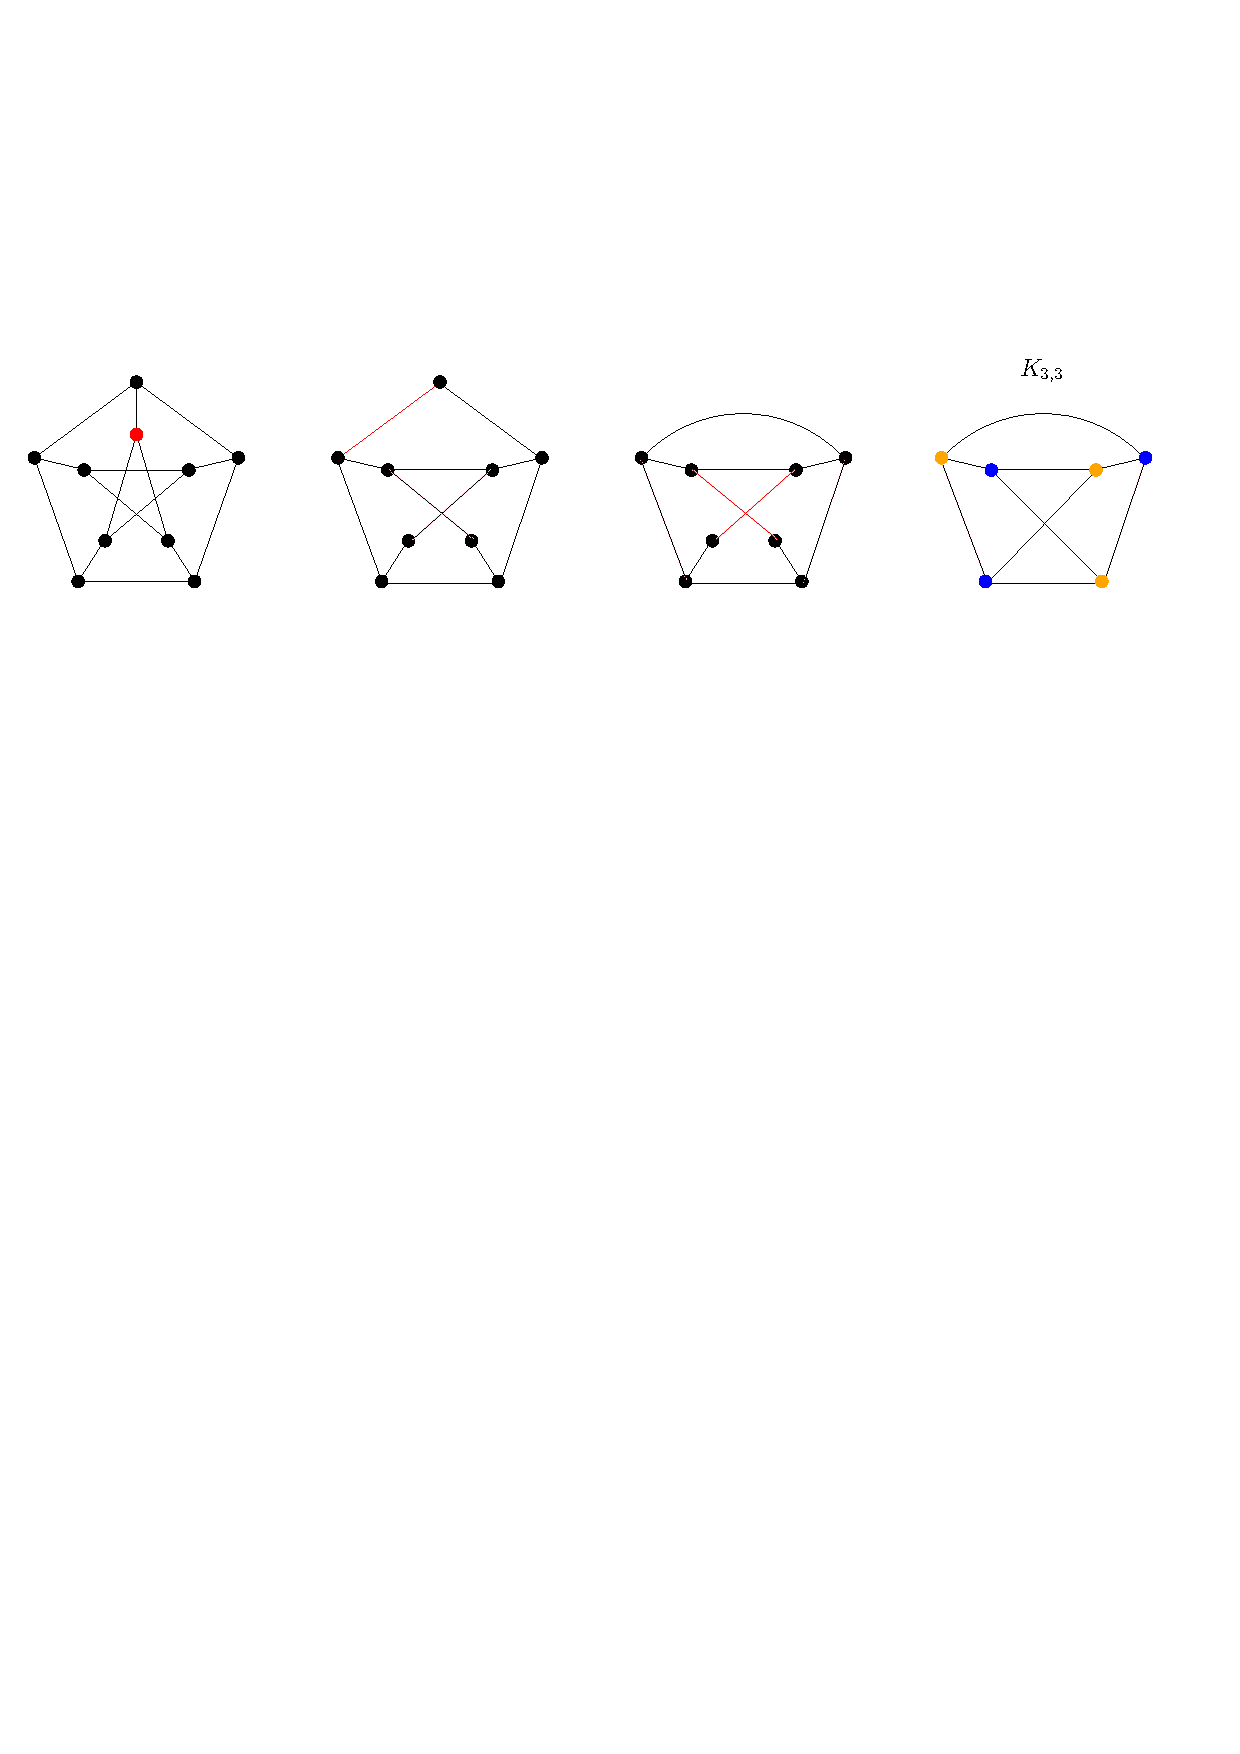
\includegraphics[width=0.9\linewidth]{figures/petersen-graph-nonplanar.pdf}
    \caption{First, take the subgraph by removing the red vertex and edges connected to it. Then, contract the red edges. We notice that after these steps, we get a graph minor that is isomorphic to $K_{3,3}$.}
    \label{fig:petersen-graph-nonplanar}
\end{figure}

\section{Formalizing Planrity Using Topology (not covered in class)}

\end{document}